\chapter{Grundlagen neuronaler Netze}
\label{kapitel_neuralnetworks}

In diesem Abschnitt werden Künstliche Neuronale Netze\cite{dayhoff1990neural}, kurz KNN, als Forschungsgegenstand der Informatik eingeführt und deren mathematischen Grundlagen präzisiert. 
Sie stellen informationsverarbeitende Systeme nach dem Vorbild von tierischen beziehungsweise menschlichen Gehirnen dar und bestehen aus Neuronen in gewissen Zuständen und Schichten, die über gewichtete Verbindungen miteinander gekoppelt sind. Jene Gewichte sind als freie Parameter des neuronalen Netzes zu verstehen und können während des Trainingsprozesses so angepasst werden, um eine entsprechende Aufgabe zu lösen.  
Gelingt dies, so können neuronale Netze genutzt werden, um bestimmte Muster in Daten, typischerweise in Bildern, Audio oder Stromdaten, effizient zu erkennen\cite{pandya1995pattern, pao1989adaptive, urbaniak2021quality}.
Sie eignen sich daher für viele typischen Aufgaben des maschinellen Lernens, beispielsweise für die Klassifikation digitalisierter Objekte.

Im ersten Abschnitt wird das Perzeptron\cite{rosenblatt1958perceptron} als Grundeinheit eines neuronalen Netztes eingeführt. 
Im folgendem Abschnitt wird das Konzept der Multi-Layer-Perzeptronen\cite{werbos1988generalization} durch die Kopplung mehrerer Perzeptronen mit bestimmten Übertragungs- und Aktivierungsfunktion in einem Netz erläutert. Diese Repräsentierung eines KNN wird im weiteren Verlauf dieser Arbeit genutzt. 

\section{Das Perzeptron}
\label{perzeptron_abs}
Zunächst wird das \textit{Perzeptron} ähnlich wie in Minsky \cite{minsky2017perceptrons} als fundamentaler Baustein eines neuronalen Netzes eingeführt. Das Perzeptron stellt im Allgemeinen ein erstes trainierbares Modell dar und wird oft als Basis moderner KNN angeführt. 
\begin{defi}[Perzeptron]
    \label{def_neuron}
    Für eine gegebene Funktion $\psi: \RR \rightarrow \RR$, einen Vektor $w \in \Rnv$ und ein Skalar $\theta \in \RR$ wird die Funktion 
    \[ \
    \Psi: \RR^n \rightarrow \RR, \; \; \; x \mapsto \psi(w^T x +\theta)=:y,
    \]
    \textit{Perzeptron} genannt. Mit $x \in \Rnv$ wird die vektorwertige Eingabe und mit $y \in \RR$ die skalare Ausgabe des Perzeptrons bezeichnet. Dabei ist mit $w^Tx=\sum_{i=1}^n w_i x_i$ das Standardskalarprodukt im euklidischen Vektorraum $\Rnv$ gemeint.
\end{defi}
Bei der Wahl der Funktion $\psi$ gibt es mehrere Möglichkeiten. Wird wie in Minsky\cite{minsky2017perceptrons} die Heavyside-Funktion
\begin{equation*}
    \psi: \RR \rightarrow \RR, \; \; \;
    \psi(x)=\begin{cases}
       1 &, x \geq 0 \\
       0 &, \text{sonst}
    \end{cases}
\end{equation*} 
genutzt, kann das Perzeptron als binärer Klassifikator wie in \ref{abs_linear_trenn} interpretiert werden. Dabei dient $w$ als trennende Hyperebene und $\theta$ wird als zugehöriger Bias bezeichnet. 

Für ein Klassifikationsproblem, bei dem die Klassen nicht linear trennbar sind, scheitern diese einfachen Perzeptronen. Hier wird oft das zweidimensionale XOR-Problem angeführt, bei denen die Punktmengen $P_{-1}=\{(0,0),(1,1)\}$ und $P_{1}=\{(1,0),(0,1)\}$ getrennt werden sollen. Um solche Aufgaben zu lösen, ist es notwendig, mehrere Perzeptronen geschickt zu verknüpfen, um komplexe Entscheidungsgrenzen zu erhalten.

\section{Multi-Layer-Perzeptron}
In dieser Arbeit wird ein Künstliches Neuronales Netz als eine Menge von Perzeptronen, die in gewissen Schichten partitioniert und miteinander verbunden sind, notiert. Diese sogenannten \textit{Multi-Layer-Perzeptronen}, kurz MLP,  gelten als erste tiefe neuronale Netze und sind seit den späten 1980er Gegenstand der Forschung\cite{bourlard1990links,bounds1988multilayer,MLPbook}. Zunächst sind einige Definition notwendig, um eine lesbare Notation von MLPs zu geben.

\begin{defi}[Übertragungsfunktion]
    \label{def_net}
    Für eine gegebene Matrix $W \in \RR^{n \times m}$ und einen Vektor $b \in \RR^m$ ist 
    \[ 
    \Psi^{W,b}: \RR^n \rightarrow \RR^m, \; \; \; x \mapsto W^T x +b
    \]
    als Übertragungsfunktion definiert. Der Vektor $y=\psi^{W,b}(x) \in \RR^m $ wird auch als Netzeingabe bezeichnet.
\end{defi}
Hierbei wird der wählbare Parameter $W$ Gewichtsmatrix und $b$ Biasvektor genannt, welche die Netzeingabe eines Eingabevektors $x \in \RR^n$ auf lineare Art und Weise beeinflussen. Um auch nichtlineare Zusammenhänge darzustellen, werden Aktivierungsfunktionen benutzt.

\begin{defi}[Aktivierungsfunktion]
    \label{def_act_f}
    Eine stetige, monoton steigende Funktion und nicht notwendigerweise lineare Funktion $\psi: \RR \rightarrow \RR$ wird als Aktivierungsfunktion bezeichnet.
\end{defi}
Es sei erwähnt, dass auch nicht monotone Aktivierungsfunktionen genutzt werden können, beispielsweise radiale Basisfunktionen\cite{radialbasis}, welche jedoch in dieser Schrift nicht weiter von Interesse sind.
Typische Aktivierungsfunktionen welche heutzutage verwendet werden sind:
\begin{align*}
    \text{Identität}: \; \;\psi(x)&=x, \\
    \text{Logistische Funktion}: \; \;\psi(x)&=\frac{1}{1+\mathrm{e}^{-x}}, \\
    \text{Tangens Hyperbolicus}: \; \;\psi(x)&=\tanh(x), \\
    \text{ReLU (rectified linear unit)}: \; \;\psi(x)&=\max\{0,x\}.
\end{align*}

Bei Klassifikationsproblemen wird oft die \textit{Softmax}-Funktion\cite{denker1990transforming} genutzt, welche die gesamte Eingabe berücksichtigt. 

\begin{defi}[Softmax]
    Für $x \in \RR^n$ wird die Funktion $\psi: \RR^n \rightarrow (0,1]^n$ mit 
    \[
        \psi(x):=\left(\frac{\mathrm{e}^{x_1}}{\sum_{i=1}^n \mathrm{e}^{x_i}}, \ldots,\frac{\mathrm{e}^{x_n}}{\sum_{i=1}^n \mathrm{e}^{x_i}} \right)^T
    \]
    als Softmax-Funktion definiert. Da sich die Einträge des Vektors $\psi(x)$ zu Eins summieren, kann die Aktivierung als eine Verteilung interpretiert werden, welche die Wahrscheinlichkeiten für bestimmte Klassenzugehörigkeiten angeben.  
\end{defi}

Für den späteren Trainingsprozess ist es nützlich, die Ableitung der verwendeten Aktivierungsfunktion, sofern sie exisitiert, zur Verfügung zu haben.

\begin{lem}
    \begin{itemize}
        \item[(i)] Für die ReLU $\psi(x)=\max\{0,x\}$ gilt
         \[\psi'(x)=\begin{cases}
            0 &, x <0 \\
            1 &, x >0
        \end{cases}. 
        \]
        An der Stelle 0 ist die Ableitung nicht definiert und wird oft mit $\psi'(0)=\frac{1}{2}$ festgelegt.
        \item[(ii)] Für die logistische Funktion $\psi(x)=\frac{1}{1+\mathrm{e}^{-x}}$ gilt
        \[ 
            \psi'(x)=\psi(x)(1-\psi(x)) 
        \]
        für alle $x \in \RR$.
        \item[(iii)] Für den Tangens Hyperbolicus $\psi(x)=\tanh(x)$ gilt
        \[ 
            \psi'(x)=1-\psi^2(x) 
        \]
        für alle $x \in \RR$.
    \end{itemize}
\end{lem}

\begin{bem}
    Ist $\psi$ eine Aktivierungsfunktion, so wird für $x \in \RR^n$ mit 
    \[\psi(x):=\left(\psi(x_1), \ldots, \psi(x_n)\right)^T \in \RR^n
    \]
    der Vektor bezeichnet, welcher sich durch die elementweise Auswertung der Aktivierungsfunktion $\psi$ ergibt. 
\end{bem}

Ähnlich der Definition des Perzeptron \ref{def_neuron} wird nun eine Schicht als Verknüpfung von Übertragungsfunktion und Aktivierungsfunktion definiert.

\begin{defi}[Schicht]
    Ist $\Psi^{W,b}$ eine Übertragungsfunktion und $\psi$ eine Aktivierungsfunktion, so wird das Paar $(\Psi^{W,b}, \psi)$ als Schicht $\mathcal{S}$ bezeichnet. Für eine vektorwertige Eingabe $x \in \RR^n$ ist die Ausgabe $y \in \RR^m$ der Schicht durch
    \[y=\psi \circ \Psi^{W,b}(x)= \psi\left(\Psi^{W,b}(x)\right)
        \] 
        gegeben. Die Komponenten $y_i$ werden für $1 \leq i \leq n$ Neuronen der Schicht $\mathcal{S}$ genannt und gleichen jeweils der Ausgabe eines einfachen Perzeptrons wie in Definition \ref{def_neuron}. 
\end{defi}
Im Hinblick auf MLPs werden nun mehrere Schichten so verbunden, dass die Ausgabe einer Schicht $\mathcal{S}_l$ als Eingabe einer darüberliegenden Schicht $\mathcal{S}_{l+1}$ für ein $l \in \mathbb{N}$ dient. Dementsprechend werden die Dimensionen der beteiligten Gewichtsmatrizen und Biasvektoren passend gewählt. 
Um die Notation übersichtlich zu halten, bezeichne $\Psi^{W^{(l)},b^{(l)},\psi_{l}}$ die Schicht $\mathcal{S}_l$ mit $\Psi^{W^{(l)},b^{(l)},\psi_{l}}(x):= \psi_{l} \left(\Psi^{W^{(l)},b^{(l)}}(x)\right)$.

\begin{defi}[Multi-Layer-Perzeptron, vgl. gruening]
    Für eine gegebene Anzahl $l \in \mathbb{N}, \; l>1$ von Schichten $\Psi^{W^{(1)},b^{(1)},\psi_{1}}, \ldots, \Psi^{W^{(l)},b^{(l)},\psi_{l}}$ bezeichne $s_l \in \mathbb{N}$ die Anzahl der Neuronen in Schicht $l$. Für eine Eingabe $x \in \RR^{s_0}$ lässt sich die Ausgabe $y \in \RR^{s_l}$ eines Multi-Layer-Perzeptron  $\Lambda_l: \RR^{s_0} \rightarrow \RR^{s_l}, \; x \mapsto y$ mit $l$ Schichten durch
    \[
        y=\Psi^{W^{(l)},b^{(l)},\psi_{l}} \circ \ldots \circ \Psi^{W^{(1)},b^{(1)},\psi_{1}}(x)
    \]
    berechnen. Die Eingabeschicht $\mathcal{S}_0$ besitzt keine Parameter $W$ und $b$ und besteht nur aus dem Eingabevektor $x \in \RR^{s_0}$. Die letzte Schicht $\Psi^{W^{(l)},b^{(l)},\psi_{l}}$ wird als Ausgabeschicht bezeichnet. Die Funktionsauswertung $\Lambda_l(x)$ für eine Eingabe $x$ wird Vorwärtsrechnung, engl. \textit{forward propagation}, genannt.
\end{defi}
\begin{equation*}
    \label{logf}
    T(x)=\frac{1}{1+\mathrm{e}^{-x}}
\end{equation*}

verwendet. An dieser Stelle sei erwähnt, dass für die Ableitung der logistischen Funktion für alle $x \in \RR$ der Zusammenhang
\begin{equation*}
    \label{difflogf}
    T^{\prime} (x)=T(x)(1-T(x)) 
\end{equation*}

gilt. Diese Eigenschaft wird später noch ausgenutzt. Nun soll die Arbeitsweise eines Neurons erläutert werden. Dabei bezeichne $x:=(x_1, \ldots, x_n)^{T} \in \Rnv$ einen Eingabevektor oder auch Merkmalsvektor der Dimension $n$, der aus einem gewissen digitalisierten Objekt $O$ erzeugt wird. Für das Neuron $v$ wird die Netzeingabe $net(v) \in \RR$ und die Ausgabe $out(v) \in \RR$ gemäß
\begin{align*}
    \label{neuronoutput1}
    net(v) &= \sum_{i=1}^n w_i x_i, \\
    out(v) &= T(net(v)-\theta)
\end{align*} 
berechnet und anschließend eine Aktivierung $y=out(v)$ zugeordnet. In der Abbildung \ref{funktionsweise_neuron} ist das abstrakte Neuron mit den entsprechenden Bestandteilen wie in Definition \ref{def_neuron} und deren Zusammenwirken dargestellt.

\begin{figure}[h]
    \label{funktionsweise_neuron}
    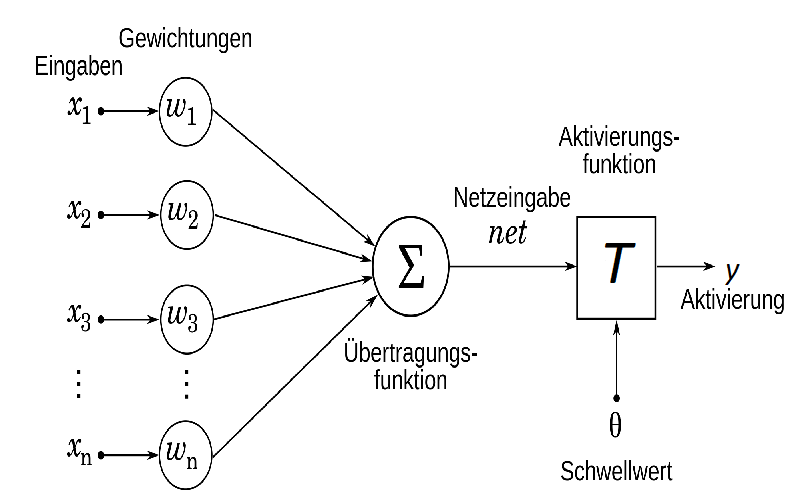
\includegraphics[width=0.8\textwidth]{pics/chapter_neuralnetworks/NeuronModel_wiki_n.png}
    \centering
    \caption{Funktionsweise eines Neurons mit entsprechender Notation aus Definition \ref{def_neuron}.}
\end{figure}

\section{Mehrschichtige Feed-Forward-Netze}